\documentclass[a4paper,10pt]{article}
\usepackage[utf8]{inputenc}
\usepackage{hyperref}
\usepackage{graphicx}

%opening
\title{Auslagerung der Ausführung von Methoden der HYPRE Bibliothek in ein Cloudsystem
Recherche und Literaturverzeichnis}
\author{Thomas Rückert}

\begin{document}

\maketitle
\newpage

\begin{abstract}

\end{abstract}

\newpage

\tableofcontents

\newpage

\section{Informationssammlung und Einführung in die relevanten Themen}

\subsection{Recherche zum Thema Cloud}

\subsubsection{Einführung und Grundbegriffe zu Cloudcomputing}

Entwicklung von monolitischen Systemen zu verteilten Anwendungen (SOA, Client/Server).
Ermöglicht Auslagerung kostenpflichtiger Berechnungen auf Server, `schwacher` Client kein Problem mehr.
Serverlast kann bei Anwendungen stark schwanken.
Zum Beispiel periodische Schwankungen Tag vs Nacht.
Klassischer Server muss die hohe Last stemmen, hat dann in anderen Perioden starken leerlauf.
Einmalige, sehr hohe Last bei besonderen Situationen (zum Beispiel durch einmalige, nicht wiederkehrende Sportevents wie Olympia/WM).
Klassischer Server könnte in diesem Zeitraum komplett ausfallen.
Cloud soll dynamische Resource sein, die sich je nach Bedarf skalieren kann.

\begin{figure}[htbp]
\centering
\caption{Übersicht Grundlagen Cloud Computing}
\label{fig:cloudComputingOverview}
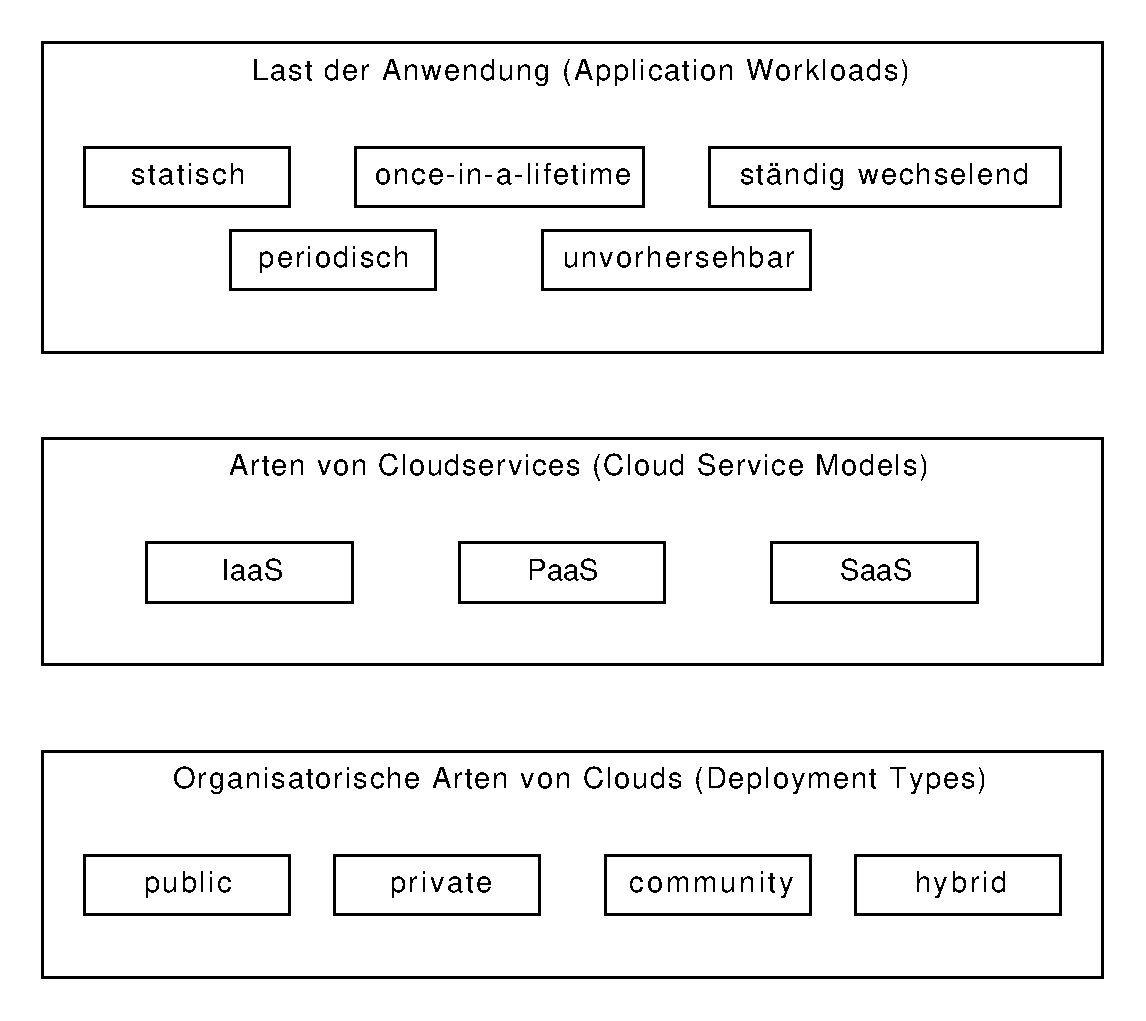
\includegraphics[width=\textwidth]{graphics/cloudComputingOverview.pdf}
\end{figure}

Im Folgenden werden die eben kurz angeschnittenen Eigenschaften von Cloudsystemen näher betrachtet.
Ein Übersicht dazu ist in Abbildung \ref{fig:cloudComputingOverview} gegeben.

\paragraph{Verteilung der Last von Anwendungen}

Im Buch Cloud Computing Patterns von Christoph Fehling wird die Verteilung von Last in die folgenden Kategorien eingeteilt:

\begin{itemize}
 \item static workload
 \item periodic workload
 \item once-in-a-lifetime workload
 \item unpredictable workload
 \item continuously changing workload
\end{itemize}

\textbf{Static workload} beschreibt eine nicht oder nur minimal schwankende Last.
\textbf{Periodic workload} hat dagegen wiederkehrende Schwankungen. Diese können zum Beispiel von der Tageszeit abhängig sein.
Ein \textbf{Once-in-a-lifetime workload} ist eine einmalige Lastspitze.
\textbf{Unpredictable workload} liegt vor, wenn sich die Last ständig, jedoch unregelmäßig und zufällig verändert, sodass diese nicht vorhersehbar ist.
\textbf{Continuously changing workload} verändert sich in linear steigend oder fallend.

\subsubsection{NIST definition introduces five fundamental properties that characterize a cloud offering [CloudcomputingPatterns chap. 1.1]}

\begin{itemize}
 \item On-demand self-service
 \item Broad network access
 \item Measured service (pay-per-use)
 \item Resource pooling
 \item Rapid elasticity
\end{itemize}

\paragraph{On-demand self-service}
`Provisioning` und `decomissioning` als Aktivitäten zum Hinzufügen oder Entfernen von weiteren Ressourcen.
Das kann durch Benutzer über grafische oder Kommandozeilenschnittstellen geschehen oder automatisiert über eine API.
\paragraph{Broad network access}
Ein starkes Netzwerk [genauer definieren] ist essentiell um eine Verbesserung durch die Auslagerung von Berechnungen zu erreichen. 
So kann Zugriffszeit auf Daten weniger abhängig von ihrem pysikalischen Speicherort werden.
\paragraph{Measured service (pay-per-use)}
Durch die Nutzung von Cloudsystemen kann man stark von der Flexibilität der Ressourcen profitieren.
Diese Flexibilität muss sich auch im Bezahlmodell widerspiegeln.
\paragraph{Resource pooling}
Ein Cloudsystem benötigt einen (großen [genauer definieren]) Pool an Ressourcen.
Nur so kann Flexibilität für die Nutzer gewährleistet werden.
Um eine Austauschbarkeit der Ressourcen zu ermöglichen muss eine homogene Nutzung der Ressourcen existieren. [warum? flexible Nutzung, Kosten]
\paragraph{Rapid elasticity}
Elastizität von Cloudsystemen ermöglicht eine Effiziente Zuweisung von Ressourcen auf die Nutzer.
Der Ressourcepool muss dynamisch unter den Nutzern aufgeteilt werden können.

\subsubsection{IDEAL cloud-native applications [CloudcomputingPatterns chap. 1.2]}

\begin{itemize}
 \item Isolated state
 \item Distribution
 \item Elasticity
 \item Automated management
 \item Loose coupling
\end{itemize}

\paragraph{Isolated state}
Cloudanwendungen und ihre Komponenten sollten zustandslos sein.
Jede Ressource die zustandslos ist kann deutlich einfacher entfernt oder hinzugefügt werden als eine Ressource mit einem Zustand.
So können aufeinander folgende Interaktionen eines Nutzers beliebig auf verschiedene Ressourcen verteilt werden.
Eine Ressource die beispielsweise die erste Interaktion getätigt hat wird für weitere Interaktionen nicht mehr benötigt.
\paragraph{Distribution}
Cloudsysteme können auf viele verschiedene Standorte verteilt sein.
In jedem Fall bestehen sie aus vielen verschiedenen Ressourcen.
Anwendungen sollten daher aus mehreren Komponenten bestehen, die auf verschiedene Ressourcen verteilt werden können.
\paragraph{Elasticity}
Horizontale Skalierung statt vertikaler Skalierung:
Anwendung soll vom Hinzufügen weiterer Ressourcen profitieren können (horizontal).
Es soll nicht nur die `Verbesserung` einer Ressource eine bessere performance ermöglichen (vertikal).
Die Stärke von Cloudsystemen ist die dynamische Zuweisung von Ressourcen.
Cloudanwendungen müssen daher horizontal skalieren, also eine Parallelisierbarkeit vorweisen.
\paragraph{Automated management}
Durch die Elastizität können Ressourcen von Cloudanwendungen während der Laufzeit ständig hinzugefügt und entfernt werden.
Diese Aktionen sollten aufgrund von Monitoring der Systemlast ausgelöst werden.
Damit die Verwaltung der Ressourcen jederzeit schnell und entsprechend der aktuellen Lage stattfindet sollte sie automatisiert sein.
\paragraph{Loose coupling}
Da sich die verfügbaren Ressourcen der Anwendung während der Laufzeit ändern können sollten Komponenten möglichst unabhängig voneinander sein.
Das reduziert die Fehleranfälligkeit für die Fälle in denen Komponenten kurzzeitig nicht verfügbar sind. [wie?]
Da verteilte Anwendung diese Eigenschaft aufweisen sind Technologien wie Webservices, SOA, asynchrone Kommunikation relevant für Cloudanwendungen. [Technologien etwas weiter ausführen]

\subsubsection{Arten von Cloud}

\paragraph{Cloud Service Models}

\begin{itemize}
 \item Infrastructure as a Service (IaaS)
 \item Platform as a Service (PaaS)
 \item Software as a Service (SaaS)
\end{itemize}

\textbf{Infrastructure as a Service} gibt einem Zugang zu Netzwerk, Computern (unter umständen virtuell) und Speicher.
Es ist daher sehr nah an den schon länger existierenden und bekannten Hosted Server Lösungen. [wie zum beispiel, kurz erläutern]
\textbf{Platform as a Service} dageben entfernt die Notwendigkeit die unterliegende Infrastruktur zu verwalten.
Das betrifft Hardware sowie die Betriebssystemebene.
Man erhält eine Umgebung in der man seine Anwendung ausführen kann, ohne sich um Themen wie Updates, Kapazitäten von Speicher und anderen Ressourcen oder ähnliche typische Adminaufgaben kümmern zu müssen.
\textbf{Software as a Service} stellt ein Cloudmodell dar, welches sich eher an Endnutzer richtet.
Man erhält Zugriff auf eine Komplette Anwendung, wie zum Beispiel einen Mailserver.
Bei dieser Variante muss sich der Nutzer um keinerlei Aufgaben der Verwaltung der Software kümmern.

\paragraph{Organisatorische Arten von Clouds (Deployment Types)}

\begin{itemize}
 \item public
 \item private
 \item community
 \item hybrid
\end{itemize}

Eine \textbf{public cloud} ist für jeden verfügbar.
Eine \textbf{private cloud} dagegen nur für ein einziges Unternehmen oder einen Nutzer (od. Interessengemeinschaft).
Eine \textbf{community cloud} liegt zwischen den beiden ersten Varianten. 
Sie ist in der Regel für eine Menge von Unternehmen verfügbar.
Das kann notwendig werden, falls die Unternehmen an einem gemeinsamen Projekt arbeiten.
Bei \textbf{hybrid clouds} ist von mehreren Clouds die Rede.
Diese können aus verschiedenen Arten bestehen und sind untereinander verbunden.
So können sich unterschiedliche Anwendungen unter eigenständigen Umgebungen Informationen austauschen und interagieren.

\subsubsection{Cloudsysteme}

\paragraph{Verfügbare Cloudsysteme}

Vergleich in Tabelle

\paragraph{Open Source Cloudsystem für private Clouds}

\begin{itemize}
 \item openstack \url{https://www.openstack.org/}
 \item apache cloudstack \url{https://cloudstack.apache.org/}
 \item a guide to open source cloud \url{http://www.tomsitpro.com/articles/open-source-cloud-computing-software,2-754.html}
 \item 5 open source cloud platforms \url{http://solutionsreview.com/cloud-platforms/open-source-cloud-platforms-enterprise/}
\end{itemize}

\subsubsection{Ressourcen}

\begin{itemize}
 \item amazon aws \url{https://aws.amazon.com/types-of-cloud-computing/}
 \item BOOK: cloud computing patterns \url{https://katalog.bibliothek.tu-chemnitz.de/Record/0012763915}
\end{itemize}

\subsection{HYPRE - Überblick über die Bibliothek}

HYPRE ist eine freie Software von Lawrence Livermore National Laboratory.
Es ist unter der GNU Lesser General Public License (Free Software Foundation) Version 2.1 lizensiert.
Der Funktionsumfang von HYPRE umfasst 'Scalable Linear Solvers and Multigrid Methods'.
Es steht als Bibliothek für die Sprachen C (nativ) und FORTRAN bereit.
Die aktuellste Version 2.11.1 ist seit dem 09.06.2016 verfügbar.
Bis zur vorletzten Version 2.10.1 wurde HYRPE auch mit dem Babel Interface bereit.
Dieses bot die Möglichkeit HYPRE von anderen Sprachen als C und FORTRAN zu nutzen.
So wurde im User Manual die Verwendung aus der Sprache Python beschrieben.

-performance?

\subsubsection{Funktionsumfang allgemein}

Wie bereits erwähnt wird der Funktionsumfang von HYPRE als 'Scalable Linear Solvers and Multigrid Methods' beschrieben.

-was heist das? was genau kann man lösen?

\subsubsection{Funktionsweise}

wie löst sie die probleme (groben einblick in die funktionsweise der methoden, falls möglich)

-wie funktioniert das? (lässt sich das beantworten)

\subsubsection{Verwendung}

-Beispiele. Benutzung.

\subsubsection{Ressourcen}

\begin{itemize}
 \item Übersicht Publikationen: \url{http://computation.llnl.gov/projects/hypre-scalable-linear-solvers-multigrid-methods/publications}
 \item Pursuing scalability for hypre's conceptual interfaces \url{http://dl.acm.org/citation.cfm?doid=1089014.1089018}
\end{itemize}

\subsection{weiteres [umbenennen]}

\begin{itemize}
 \item c/c++ json lib benchmarks \url{https://github.com/miloyip/nativejson-benchmark}
 \item nur innerhalb der cloud (ungeeignet): Light-weight remote communication for high-performance cloud networks \url{http://ieeexplore.ieee.org/document/6483669/}
 \item Performance Analysis of High Performance Computing Applications on the Amazon Web Services Cloud \url{http://ieeexplore.ieee.org/abstract/document/5708447/}
\end{itemize}

\paragraph{rpc}

\begin{itemize}
 \item understanding rest and rpc for http \url{https://www.smashingmagazine.com/2016/09/understanding-rest-and-rpc-for-http-apis/}
 \item Implementing remote procedure calls \url{http://dl.acm.org/citation.cfm?id=357392}
 \item c++ json-rpc lib \url{https://github.com/cinemast/libjson-rpc-cpp/}
\end{itemize}


\newpage

\section{Vergleich verschiedener Technologien und Werkzeuge für den Einsatz bei der Implementierung}

\subsection{'private' vs 'public' Cloud}

\begin{itemize}
 \item gibt es open source cloud systeme? welche?
 \item welche public clouds gibt es (zB aws, windows azure, adobe creative)
 \item was sind unterschiede (neben dem access, zB performance?)
\end{itemize}

\subsection{Technologie}

\begin{itemize}
 \item welche Werkzeuge für die kommunikation zwischen client und cloud
 \item rpc, socket, service ...
 \item abwägen zwischen performance, aufwand ...
 \item welche framework könnten genutzt werden
\end{itemize}


\subsection{Cloudtyp}

wird evtl schon teilweise in abschnitt 1 (allgemeines zur cloud) abgedeckt

\begin{itemize}
 \item Infrastructure as a Service (IaaS)
 \item Platform as a Service (PaaS)
 \item Software as a Service (SaaS)
 \item aber entscheidend: wie eignen sich diese typen für `unsere` Implementierung
\end{itemize}

\subsection{Sprache}

\begin{itemize}
 \item hardware-nah: C/C++ (bessere performance)
 \item vs netzwerknah: (bessere möglichkeiten die kommunikation zu Implementieren)
 \item kann eine hybridform eingsetzt werden? 
 zB (micro-)service: bib in c kommuniziert mit client-backend in php, dieses führt die calls zum server aus
\end{itemize}

\newpage

\section{Zukünftige, weiterführende Arbeiten}

eventuell werden Teile von hier in die aktuelle Arbeit verschoben

\begin{itemize}
 \item Skalierbarkeit der Cloud (einsetzen)
 \item Vorteile der Auslagerung:
  \begin{itemize}
    \item performance
    \item speicher
    \item lösbarkeit (nur remote überhaupt lösbar)
  \end{itemize}

\end{itemize}


\end{document}
